\chapter{Problem analysis}
We need to analyze and describe our problem domain.
This will be achieved by identifying different kinds of user roles, specifying user requirements, creating use cases, and describing those use cases via use case scenarios.

\section{User roles}
There are two types of users who will come in contact with the application.
The first type is a \textbf{restaurant}, more specifically its employee who is responsible for creating menus.
This user needs to have a basic understanding of how to use a computer or smartphone and a web browser.
The application will help restaurant employees to create menus online, and will let them specify allergens contained in each meal of a menu.

The second type of users are the restaurant \textbf{guests}.
They, too, need to have a basic understanding of how to use a computer or smartphone and a web browser.
The application will enable a restaurant guest to create a personal profile where they will specify their food preferences, including allergies and diets.
When a guest will visit a restaurant, the application will enable them to filter out meals in the restaurant's menu which they are automatically not interested in ordering based on their profile.

\section{User requirements vocabulary}
It is good practice to use language consistently throughout all requirements, and that is why we are going to resolve what the keywords in requirements mean.
If a requirement states that the application \textbf{shall} do something, then it means that the requirement is mandatory for the application and has to be addressed in the design phase which follows after this chapter. 
The word \textbf{should} is for desired requirements which are not critical for the application's functionality.
Last but not least, usage of the word \textbf{must} indicates a domain constraint.
Also, we will substitute the user role restaurant for \emph{restaurant employee} where it will be more convenient.
In the next two sections, we are going to specify all user requirements. 

\section{Functional requirements}
We will look at requirements from the application's user point of view.
That is why we will organize the requirements based on which user role defines them.
If a requirement is defined by both user roles, it will be listed outside the role specific sections.
The following list of functional and non-functional requirements is inspired by an interview done with a restaurant\footnote{\url{https://pizzabudca.sk/}  \label{fnlabel}} employee.

\subsection{Restaurant requirements}
\begin{description}
    \item [Req. 1.1:] A restaurant employee shall be able to create a menu.
    \item [Req. 1.2:] A restaurant employee shall be able to assign a created menu to a specific day.

    \emph{Rationale:} Typically, a restaurant has one menu for a day.
    \item[Req. 1.3:] A restaurant employee should be able to set a concrete menu for more than one day.

    \emph{Rationale:} A menu can be the same for several consequent days.
    \item [Req. 1.4:] The application shall enable a restaurant employee to edit a previously created menu.
    \item [Req. 1.5:] The application shall enable a restaurant employee to delete a previously created menu.
    \item [Req. 1.6:] A restaurant employee should be able to re-use a previously created menu when selecting menu for a day.
    \item [Req. 1.7:] A restaurant employee should be able to print a menu.
    \item [Req. 1.8:] A restaurant employee should be able to set a menu periodically for a certain day of the week.

    \emph{Rationale:} A menu can be the same for a certain day of the week. 
    \item [Req. 1.9:] A restaurant employee should be able to specify which Solid pod to use for storing the restaurant's data.

    \emph{Rationale:} A restaurant can have multiple Solid pods associated with its WebID.
\end{description}

\subsection{Guest requirements}
\begin{description}
    \item [Req. 2.1:] The application shall enable a restaurant guest to specify what allergies they have.
    \item [Req. 2.2:] The application shall enable a restaurant guest to specify what diets they are on.
    \item [Req. 2.3:] The application should enable a restaurant guest to specify what food and beverages they like.
    \item [Req. 2.4:] The application should enable a restaurant guest to specify what food and beverages they dislike.
    \item [Req. 2.5:] The application shall enable a restaurant guest to see a personalized menu based on the guest's profile.
    \item [Req. 2.6:] The application should be able to sort meals in a menu by whether a viewing guest can eat them according to their profile.

    \emph{Rationale:} This will allow the application to visibly divide a menu.
    \item [Req. 2.7:] The application should be able to filter out meals of a menu which a viewing guest cannot eat according to their profile.
    \item [Req. 2.8:] A guest shall be able to load a menu by specifying the IRI of the menu.
    \item [Req. 2.9:] A guest should be able to load a menu by scanning a QR code printed on the menu.

    \emph{Rationale:} The QR code will link to the application and will provide it with the IRI of the printed menu.
    \item [Req. 2.10:] A guest should be able to specify an IRI of a restaurant to browse its menus.
    \item [Req. 2.11:] The application should enable a guest to mark a restaurant as favorite.
    
    \emph{Rationale:} A guest should have a set of their favorite restaurants.
    \item [Req. 2.12:] A guest should be able to specify which Solid pod to use for storing their data.

    \emph{Rationale:} A guest can have multiple Solid pods associated with their WebID.
\end{description}

\section{Non-functional requirements}
\begin{description}
    \item [Req. 3.1:] Each item of a menu must have specified allergens contained in it.
    
    \emph{Rationale:} At least in the EU, there are laws\footnote{\url{https://eur-lex.europa.eu/legal-content/EN/ALL/?uri=celex\%3A32011R1169}  \label{fnlabel}} which mandate restaurants to list allergens contained in food they serve.
    \item [Req. 3.2:] The application should have responsive user interface and work on mobile devices as well as on desktops.
\end{description}

\section{Use cases and scenarios}
Now we are going to depict goals of users which the application will make achievable.
A use case styled with a bold border indicates that it groups together more use cases and will be further expanded later.
All use cases will be structurally described by independent use case scenarios.

\begin{figure}
    \centering 
    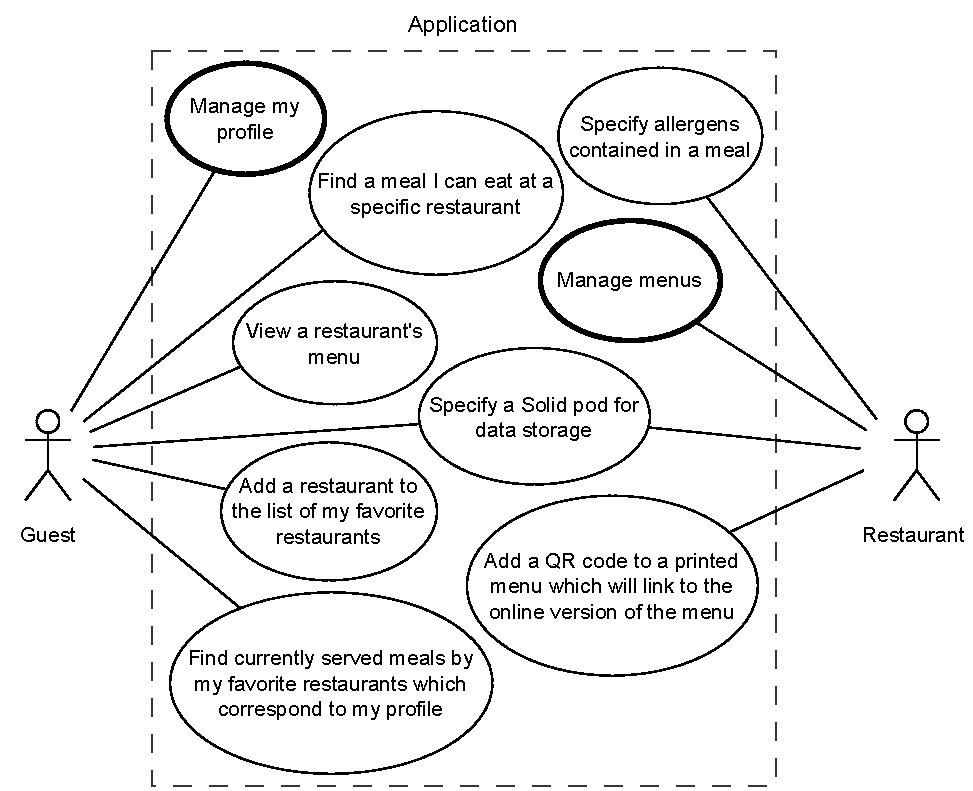
\includegraphics[width=\linewidth]{master-thesis/img/application_use_cases}
    \caption{The application's use case diagram.}
\end{figure}



\subsection{Use case scenarios}
